\documentclass[12pt]{article}
\usepackage{geometry}
\usepackage{hyperref}
\usepackage{setspace}
\usepackage{forest}
\usepackage{xcolor}
\usepackage{enumitem}
\usepackage{amsmath}
\usepackage{graphicx}

\useforestlibrary{edges}

\geometry{top=1in, bottom=1in, left=1in, right=1in}


\begin{document}

% --- Title Page ---
\begin{titlepage}
    \centering
    \vspace*{6cm}
    {\Huge\bfseries Arbitrary-Precision Arithmetic Library in Java\par}
    \vspace*{20mm}
    \vfill
    {\large Rishika Shreya Fadi \\ CS24BTECH11052\par}
\end{titlepage}

\setcounter{page}{1}
\pagestyle{plain}

% --- Table of Contents ---
\tableofcontents
\newpage

% --- Main Content ---
\section{Introduction}
\begin{spacing}{1.2}
The goal of this project is to implement an arbitrary-precision arithmetic library in Java,supporting both integer and floating-point arithmetic.\\In standard programming environments, arithmetic operations are limited by the fixed size of built-in data types such as \texttt{int}, \texttt{long}, or \texttt{double}. These limitations can lead to overflow or loss of precision when dealing with very large or highly precise numbers.\\\\
Arbitrary-precision arithmetic provides a way to perform calculations on numbers of any size or precision, constrained only by the system's memory. This project focuses on designing and implementing an arbitrary-precision arithmetic library in Java.\\
The goal is to support addition, subtraction, multiplication, and division for both integers and floating-point numbers without relying on Java's built-in \texttt{BigInteger} or \texttt{BigDecimal} classes. The library is designed from the ground up using string-based representations and custom logic to perform digit-level arithmetic operations.\\\\
Through this project, the underlying mechanisms of number representation and arithmetic could be understood clearly, and software engineering principles such as modular design, testing, and documentation to ensure project was well-structured and easy-to-maintain.\\\\
The purpose of this report is to document the design, implementation, and testing of an arbitrary-precision arithmetic library in Java. It provides a detailed explanation of the algorithms/functions that I used while building the library. The report also highlights the software engineering practices employed, such as modular design and testing.\\
Through this documentation, the goal is to share insights into the process of building a high-precision arithmetic system from scratch.


\section{Design}
The project follows a Maven-based Java structure with clear separation of source code, tests, and build outputs.

\subsection{Project Structure}


\begin{forest}
  for tree={
    font=\ttfamily,
    grow'=0,
    child anchor=west,
    parent anchor=south,
    anchor=west,
    calign=first,
    edge path={
      \noexpand\path [draw, \forestoption{edge}]
      (!u.south west) +(7.5pt,0) |- (.child anchor)\forestoption{edge label};
    },
    before typesetting nodes={
      if n=1
        {insert before={[,phantom]}}
        {}
    },
    fit=band,
    before computing xy={l=15pt},
  }
[final\_proj
  [src
    [main
      [java
        [arbitraryarithmetic
          [AFloat.java]
          [AInteger.java]
        ]
        [MyInfArith.java]
      ]
    ]
  ]
  [target
    [classes
      [arbitraryarithmetic
        [AFloat.class]
        [AInteger.class]
      ]
      [MyInfArith.class]
    ]
    [generated-sources]
    [maven-archiver]
    [maven-status]
    [arbitrary-arithmetic-1.0-SNAP.jar]
  ]
  [documentation
    [report.tex]
    [report.pdf]
  ]
  [compile\_and\_run.py]
  [pom.xml]
]
\end{forest}


   
\begin{itemize}
    \item \texttt{AInteger.java} \& \texttt{AFloat.java}: Core classes implementing \textbf{arbitrary-precision arithmetic} for integers and floating-point numbers, respectively.
    
    \item \texttt{MyInfArith.java}: \textbf{Entry point} for CLI execution, handling user input and invoking \texttt{AInteger}/\texttt{AFloat} operations.
    
    \item \texttt{src/main/java/arbitraryarithmetic}: Directory for \textbf{main source code} 
    
    \item \texttt{target/}: Maven's build output (compiled classes, JAR artifacts, and metadata)
    
    \item \texttt{pom.xml}: Maven configuration file defining dependencies and build settings
    
    \item \texttt{compile\_and\_run.py}: Utility script to automate compilation/execution
    
    \item \texttt{documentation/report.tex}: Project documentation in \LaTeX
\end{itemize}



\subsection{UML Class Diagram}
\begin{spacing}{0.2}
\begin{figure}[h]
    \centering
    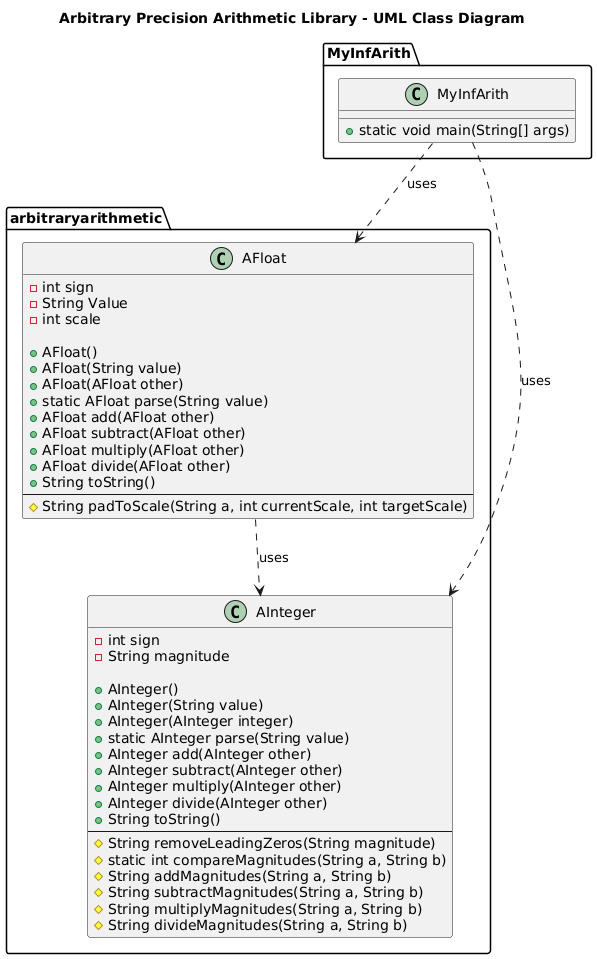
\includegraphics[width=0.5\textwidth]{UMLDiagram.png}
    \caption{UML Class Diagram for \texttt{MyInfArith , AInteger and AFloat}}
    \label{fig:your_label}
\end{figure}
\end{spacing}




\section{Implementation}
\subsection{Integer arithmetic}

\begin{itemize}[leftmargin=*]
    \item \textbf{Addition}
    \begin{itemize}
        \item Processes digits \textbf{right-to-left}
        \item Sums digits + carry from prior step
        \item Stores last digit of sum, carries forward the rest
        \item Reverses final result
        \item helper-function \texttt{addMagnitudes} is used.
    \end{itemize}

    \item \textbf{Subtraction}
    \begin{itemize}
        \item Works \textbf{right-to-left}
        \item Subtracts digits + borrow from prior step
        \item If result $< 0$, adds 10 and sets borrow $= 1$
        \item Trims leading zeros from result
        \item helper-functions \texttt{subtractMagnitudes} and \texttt{compareMagnitudes} are used.
    \end{itemize}
    \item In Addition if one of the numbers is negative then subtraction logic is implemented
    \item In Subtraction if only one of the numbers is negative then addition logic is implemented.

    \item \textbf{Multiplication}
    \begin{itemize}
        \item Processes digits right-to-left, multiplying each digit pair
        \item Stores results in a temporary array with proper digit positioning
        \item Handles carries automatically by splitting products into tens/units places
        \item Converts the final array to a string, trimming leading zeros.
        \item Sets sign positive if operands have same sign, negative otherwise.
        \item helper-functions \texttt{multiplyMagnitudes} is used.
    \end{itemize}

    \item \textbf{Division}
    \begin{itemize}
        \item Performs digit-by-digit long division on the magnitude strings.(repeated subtraction and remainder tracking)
        \item Processes the dividend left-to-right, building a "current" number
        \item Repeatedly subtracts the divisor from "current" to count quotients
        \item Appends each quotient digit and continues with the remainder
        \item Returns "0" if divisor $>$ dividend, otherwise the quotient string
        \item uses \texttt{subtractMagnitudes} and \texttt{compareMagnitudes} as helper-functions.
    \end{itemize}
    
\end{itemize}
\subsection{Floating-point arithmetic}
Basic logic: remove the decimal points and perform the operations on the numbers as if they were integers and depending on the operation add the decimal point in the result.

\begin{itemize}[leftmargin=*]

    \item \textbf{Addition}
    \begin{itemize}
        \item Equalizes decimal places by padding the shorter number with trailing zeros
        \item Treats both numbers as integers (removes decimal points)
        \item Uses \texttt{AInteger.add()} to perform exact integer addition
        \item Restores decimal position to the maximum scale among the numbers.
        \item Trims trailing zeros and limits to 30 decimal places
        \item no sign handling needs to be done because it is handled in \texttt{AInteger}.
    \end{itemize}

    \item \textbf{Subtraction}
    \begin{itemize}
        \item same padding with zeroes as addition.
        \item Treats both numbers as integers.
        \item Uses \texttt{AInteger.subtract()}.
        \item restores decimal position to the maximum scale among the two numbers.
        \item Trims trailing zeros and limits to 30 decimal places
    \end{itemize}

    \item \textbf{Multiplication}
    \begin{itemize}
        \item Sums the scales of both operands
        \item Removes decimals and treats as integers
        \item Uses \texttt{AInteger.multiply()}.
        \item Applies combined scale (decimals from both numbers).
        \item Sets sign positive if operands have same sign, negative otherwise
    \end{itemize}

    \item \textbf{Division}
    \begin{itemize}
        \item Pads numerator with 30 zeros for decimal precision
        \item final scale: relative scale difference between operands
        \item Uses \texttt{AInteger.divide()} on scaled integers.
        \item Trims trailing zeroes.
        \item Enforces 30 decimal place maximum.
        \item Handles division-by-zero error explicitly
    \end{itemize}

    
\end{itemize}

\subsection{Edge Case Handling}
\begin{itemize}
    \item Empty or Null input throws \texttt{IllegalArgumentException}.
    \item Invalid arguments like (a123, 456- etc) throws \texttt{IllegalArgumentExcpetion}.
    \item Inputs with irregular formatting (eg, .5, -.5, 000006) are all modified to proper inputs using regeX.
    \item +0, +0.0, -0, -0.0, -00000000.. inputs like these are standardized to 0.
    \item Division by Zero throws \texttt{ArithmeticException} error.
\end{itemize}

\section{Testing and Validation}
\begin{itemize}
    \item Each method (e.g., add, subtract) was tested individually with predefined inputs and expected outputs.(uploaded on Google Classroom)
    \item For larger values, outputs were compared against Java’s BigInteger or BigDecimal classes to ensure accuracy.
    \item Multiple test cases were written to cover a wide range of scenarios, such as:
    \begin{itemize}
        \item Adding two large positive integers, one positive one negative, two negative integers.
        \item Subtracting a smaller number from a larger one and vice versa.
        \item Subtracting a positive number from a negative number and vice versa.
        \item Performing floating-point addition with varying decimal lengths.
        \item Handling negative numbers and zero in different operations.
    \end{itemize}
    \item In all cases tested, the output matched the expected results
\end{itemize}

\section{Conclusion}
\subsection{What I learned}
\begin{itemize}
    \item I gained a deeper understanding of OOPS concepts such as modularity, method overloading etc.
    \item I improved my ability to write code in a more organized and clean way, making it easier to understand, test, and maintain.
    \item Gained a bit more experience in Git and Docker.
    \item Used maven for the first time.
\end{itemize}
\subsection{Conclusion}
This project helped me strengthen my programming skills and gain hands-on experience with practices in software development.

\end{spacing}
\end{document}